\chapter{Network Design}

\section{Topology}

The topology used for this lab assignment took the form of a three router set-up,
simulating an infrastructure a typical Internet Service Provider (ISP)
might have. Using three routers as opposed to a one allowed our ISP to make use
of technologies such as dynamic internal routing and iBGP in order to create a
fault-tolerant network. Joining our routers in a complete graph introduced
maximum redundancy and allowed for increased uptime as any traffic could have
been routed via an alternate path should an outage of occured on any single
device.

\begin{figure}[!ht]
    \caption{High-level Topology}
    \centering
    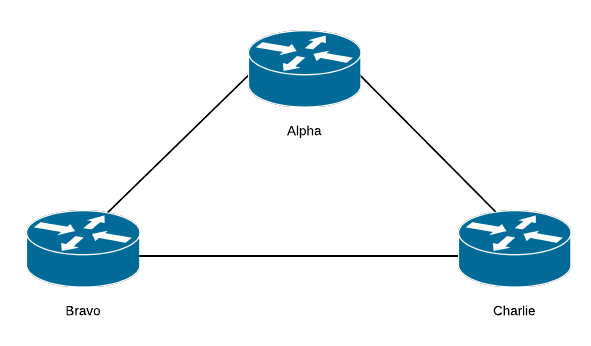
\includegraphics[width=0.8\textwidth]{images/networkTopology.png}
\end{figure}

\section{Address Allocation}
\subsection{IPv4}
For this lab exercise we were assigned the IP address space
\texttt{12.0.0.0/8}. This provided us with the ability to allocate 16.7 million
addresses, of which only a small fraction were required for our network
infrastructure. Even so, we took into account the issues that arose from the
original distribution of excessively large IPv4 network blocks to ISPs,
businesses, educational institutions, etc~\cite{ipv4alloc}\cite{internetmap}
and decided it was best to be conservative in our allocations. With this in
mind we invented three classifications of network address, each defining the
minimum subnet size deemed necessary for its purpose. These are outlined in
Figure~\ref{figure:network-alloc-1}.

\begin{figure}[!ht]
    \caption{Classifications of Network Allocations}
    \label{figure:network-alloc-1}
    \centering
    \begin{tabular}{|c|c|p{5.5cm}|}

        \hline
        \textbf{Address Type} & \textbf{Subnet Mask} & \textbf{Justification} \\

        \hline
        Customer Segment & \texttt{/24} & Allocated to downstream customers,
        who were given enough address space for 254 devices. In our network
        laptops were used to simulate customer devices. The size of this subnet
        also allowed for easy identification of the subnets' locations in our
        topology as detailed in Figure~\ref{figure:network-alloc-2}.\\

        \hline
        Point-to-point Links & \texttt{/30} & Used for links that connected two
        routers, because those links only required two IP Addresses and a
        \texttt{/30} subnet mask is the smallest mask that can provide this.

        \textbf{Note:} The connection to our provider, AS 42, was an exception
        to this and used a \texttt{/24} subnet mask as was provided by AS 42.\\

        \hline
        Loopback Address & \texttt{/32} & Used for the loopback interfaces on
        our routers. Only a single address was required and a \texttt{/32} mask
        produces this.\\

        \hline
    \end{tabular}
\end{figure}
In addition to the classification of subnets based on size, we used several IP
schemas to choose the IP values of our networks. This allowed for quick
identification of a network from its IP address without referencing our network
diagrams. For example, customer segments connected to the Alpha router had a
third octet value of 1, so it was immediately apparent that the IP address
\texttt{12.0.1.2/24} was connected to Alpha.

These conventions were decided in advance of our network build-out and helped
us diagnose issues with IP or interior routing configurations in a more
intuitive way. The exact schemas are outlined in Figure~\ref{figure:network-alloc-2}.

\begin{figure}[!ht]
    \caption{IP Schemas}
    \label{figure:network-alloc-2}
    \centering
    \begin{tabular}{|p{3cm}|p{3cm}|p{5cm}|}

        \hline
        \textbf{Schema} & \textbf{Classification} & \textbf{Identifying Feature} \\

        \hline
        \texttt{12.0.\#.0/24} & Customer Segment & The hash here dictated the
        ISP router that this address space was connected to, 1 through 3 for
        Alpha, Bravo and Charlie. This could have been scaled up to 253
        additional subnets for our Service Provider.\\
        \hline
        \texttt{12.\#.0.0/30}, where $\#> 10$ & Peer Point-to-point Link &
        The hash in these networks was the assigned number (plus 10) of the group we
        connected to on these links. This enabled us to quickly identify the
        group involved with any connectivity issues using BGP. For example, the
        link to group 3 used the subnet \texttt{12.13.0.0/30}.\\
        \hline
        \texttt{12.0.0.\#/30} & Internal Point-to-point Link &
        This hash value was a multiple of 4, starting from 0. Whilst the choice
        of hash value was effectively arbitrary, the second and third octets had
        to be 0 to avoid conflicts with our other classifications.\\
        \hline
        \texttt{12.\#.\#.\#/32} & Loopback Address & The hash here had
        the same value in all three octets of the address and dictated the
        router that this loopback was assigned to. For example,
        \texttt{12.3.3.3/32} was the loopback address of Charlie.\\

        \hline
    \end{tabular}
\end{figure}

\clearpage

\subsection{IPv6}
When allocating our IPv6 address space we took a similar approach to that of
IPv4, aiming to allocate an appropriate sized address block to each segment of
our network. As such, the classifications used were approximately the same as
for IPv4, with network segments being either a Customer Segment, Point-to-point
link or a Loopback. This is detailed in Figure~\ref{figure:network-alloc-3}.

\begin{figure}[!ht]
    \caption{Classifications of Network Allocations}
    \label{figure:network-alloc-3}
    \centering
    \begin{tabular}{|c|c|p{5.5cm}|}

        \hline \textbf{Address Type} & \textbf{Subnet Mask} & \textbf{Justification} \\

        \hline
        Customer Segment & \texttt{/36} & Allocated for downstream connections
        to our ISP's customers. A large subnet mask was used to allow for
        allocations to be broken down into subnets containing a 48-bit Global
        Routing Prefix for customer networks.\\

        \hline
        Point-to-point Links & \texttt{/64} & Used for links that directly
        connected two routers, requiring two unique IP addresses. Reasons for
        using a \texttt{/64} subnet mask are discussed below.\\
        \hline
        Loopback Address & \texttt{/128} & Used for the loopback interfaces on
        our routers. There was only a requirement for a single address, as with
        IPv4. In IPv6 a \texttt{/128} mask produces this.\\

        \hline
    \end{tabular}
\end{figure}

Customer Segments used a \texttt{/36} mask as a method of breaking down our
customer networks into more manageable blocks of addresses. The \texttt{/36}
mask allowed us to further break down our Customer Segments into IPv6 blocks
with a 48-bit Global Routing Prefix, which is a unique ID for an IPv6 address
and can be used identify both the ISP and the customer.

In Figure~\ref{figure:network-alloc-3} it is obvious that applying a
\texttt{/64} mask for point-to-point links allocates a considerable amount of
addresses to a network which would otherwise only require two. The decision to
do this was taken from RFC 4291, which dictates that ``For all unicast
addresses, except those that start with the binary value 000, Interface IDs are
required to be 64 bits long''~\cite{rfc4291}. There has been some discussion as
to whether this practise is wasteful\cite{ipv6waste}, however there are
some convincing counter arguments\cite{ipv6notwaste} and for the purposes of
this lab we have chosen to adhere to the RFC.
